\section{Approach} 
\label{approach}

Figure \ref{pipeline} visualizes the steps of our approach, which are described in detail in the following chapters.

\begin{figure}[ht]
	\centering
	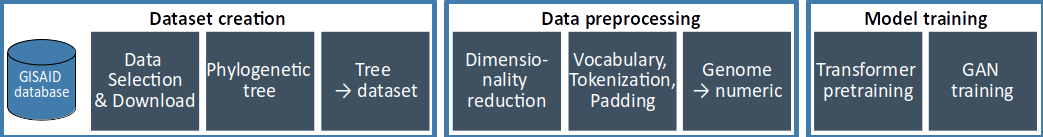
\includegraphics[width=1.0\linewidth]{figures/pipeline.png}
	\caption{Approach pipeline \cite{own representation}}
	\label{pipeline}
\end{figure}


\subsection{Dataset Creation}  \label{ch:approachA}
% Choosing latest mutations that are the most spread
% Created three types of sequence pairs: (real, real), (real, generated), (real, unreal)
% Phylogenetic tree with "Fasttree"
% Levenshtein distance
% Biopython packages?
% Final dataset metrics

As described in chapter \ref{fundamentalsC} a dataset consisting of parent-child pairs is needed to learn a \ac{ML} model for mutation prediction. The steps to create this dataset are described in the following chapters.

\subsubsection{Raw data selection from \ac{GISAID}}
\label{ch:approachAa}

In the first step of the dataset creation the raw genomes and their metadata are downloaded from \ac{GISAID}. Therefore a selection of a suitable subpart of the data is necessary. The \ac{GISAID} platform only allows the download of 5000 genomes at once. That is why we decided to focus our analysis on Germany (for one country the selection of < 5000 genomes is rather simple compared to the selection of data from multiple countries). By looking at the latest "Report on virus variants of SARS-CoV-2 in Germany" from the \ac{RKI} we decided for a time period. Figure \ref{rkiVariantDistribution} shows the distribution of different variants over time. Starting from calendar week 18 the Delta variant gradually displaces the previously widespread Alpha variant.

\begin{figure}[ht]
	\centering
	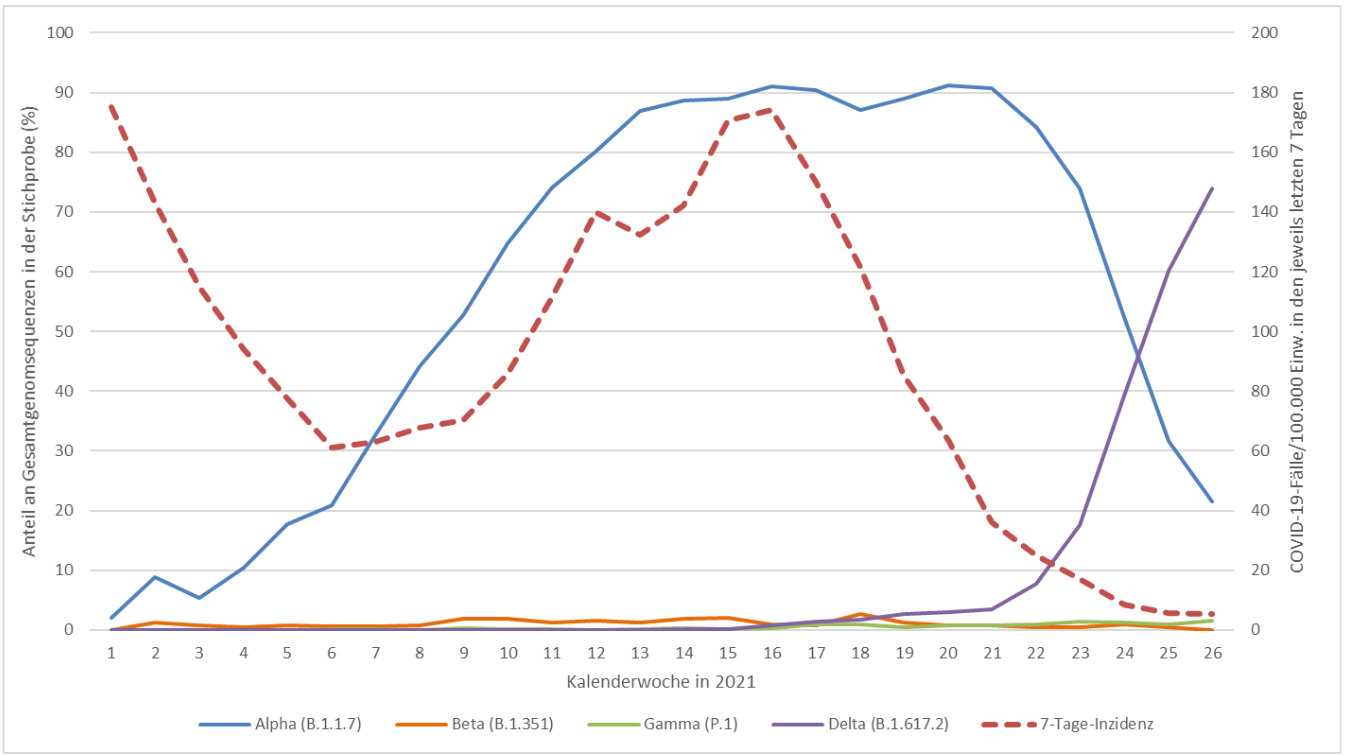
\includegraphics[width=1.0\linewidth]{figures/rkiVariantDistribution.png}
	\caption{Variant distribution in Germany over time \cite{robertkochinstituteditorBerichtVirusvariantenSARSCoV22021}}
	\label{rkiVariantDistribution}
\end{figure}

That is why we selected the data from 04.05.2021 (calendar week 18) until 15.07.2021 (calendar week 28). This results in a raw dataset of 35.818 genomes.
Each genome consists of a FASTA file containing the genomes sequence and a record in a tsv file with the metadata.

%TODO: beispiel record: genome sequence and metadata


\subsubsection{Generation of a phylogenetic tree}
\label{ch:approachAb}

As described above we need parent-child genome sequence pairs to be able to train a \ac{ML} model. Therefore we need to evaluate the ancestral relationships between the genome sequences.
As described in chapter \ref{fundamentalsA0d} this is done in biology through phylogenetic trees.
For the data preparation (e.g. alignment) and the calculation of the phylogenetic tree we use the nextstrain pipeline \cite{10.1093/bioinformatics/bty407}.
The pipeline was executed on a local computer with Intel Core i7-7500U (4*2.70GHz), NVIDIA GeForce 940MX and 16 GB RAM.
Unfortunately after two days of calculation, the nextstrain pipeline exited with an out of memory exception. That is why the amount of data is decreased. This was done through iterative reduction of the dataset size. The largest locally computable dataset consists of 11.773 genome sequences.

The generated phylogenetic tree can be seen in figure \ref{phylogeneticTree}.
%TODO: Beschreibung was man sieht

%TODO: nicer tree image?
\begin{figure}[ht]
	\centering
	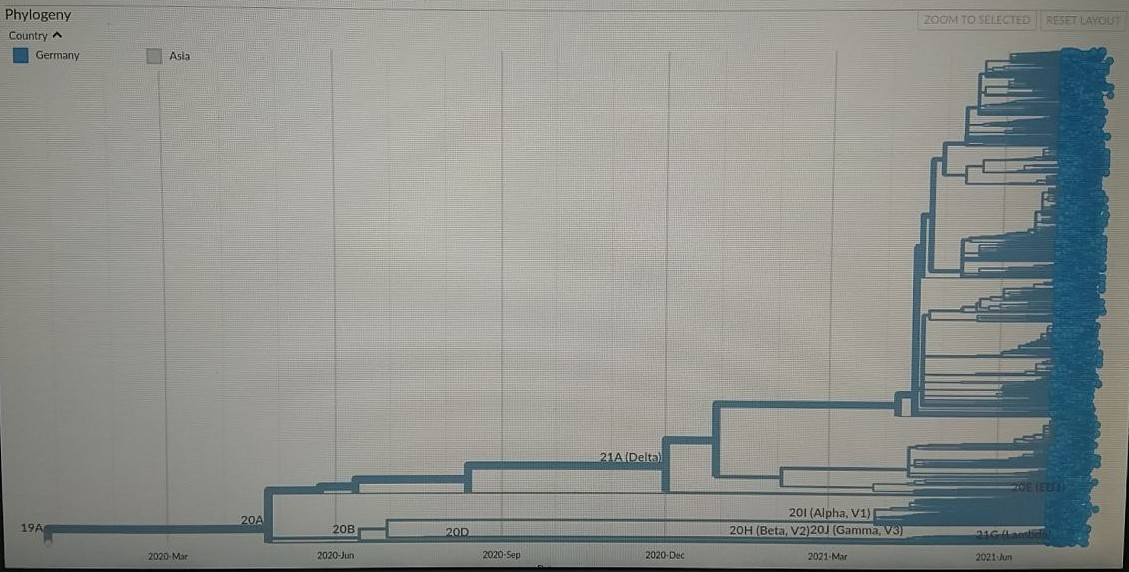
\includegraphics[width=1.0\linewidth]{figures/phylogeneticTree.jpg}
	\caption{Phylogenetic tree of our dataset \cite{own representation}}
	\label{phylogeneticTree}
\end{figure}

\subsubsection{Phylogenetic tree to dataset}
\label{ch:approachAc}

Based on the calculated phylogenetic tree the final dataset is generated. Therefore the patristic distances between all leaf nodes are calculated. From the resulting patristic distance matrix for each leaf node the most related next leaf node can be evaluated. The two leaf nodes with the smallest distance are the closest relatives to each other and therefore represent a parent-child pair. After the evaluation which leaf nodes are one parent-child pair, the question which node is the parent and which node is the child is clarified. Therefore the two nodes are sorted by their date, which is stored in the metadata file. The older genome sequence is the parent and the younger genome sequence is the child.

For calculating the patristic distance matrix we first used Dendropy (version: 4.5.2) \cite{DendroPyPhylogeneticComputing}. Again this leads to problems due to limited RAM on our local computer. As a consequence we switched to PhyloDM (version: 1.3.1) \cite{aaron_mussig_2020_4089111}, which is a library for calculating patristic distances in a memory and time efficient manner.

Finally we received a dataset containing parent-child genome sequences.

\subsection{Data Preprocessing}  \label{ch:approachB}
% TODO: Pipeline image
% Word size 3 is just a hyperparameter (see discussion of the corresponding paper)!  But maybe biologically valid because auf amino acids.
% DNA2Vec?

\subsubsection{Dimensionality reduction by selecting subpart of the genome}
\label{ch:approachBa}

The full \ac{SARS-CoV-2} genome consists of about 30.000 nucleotides. Due to the limited computing capacity on our local computers we need to reduce the dimensionality of the dataset. This is done by selecting a subpart based on the gained data insights from chapter \ref{ch:experimentsA}. In figure \ref{mutatedGeneticLoci} parts of the genome with lots of mutations are visible. Based upon this we selected 99 nucleotides (33 codons) in the range between position 21.800 and 21.899.

\subsubsection{Transform genome sequence to numeric model input}
\label{ch:approachBb}

Input to the model are numericalized codon sequences with each codon being composed of three nucleotides. Therefore one needs to build a vocabulary with all codons existing in the dataset that assigns each codon a unique number. Each genome string is therefore tokenized to codons and so far unseen codons are added to the vocabulary. The vocabulary also contains special tokens like:

\begin{itemize}
	\item \textit{<SOS>}: start of sentence
	\item \textit{<EOS>}: end of sentence
	\item \textit{<UNK>}: unknown
	\item \textit{<PAD>}: padding
\end{itemize}

A codon is encoded as unknown in case at least one nulceotide is unknown or at least one padding character is contained. Only in the special case of three padding characters the padding token is returned. 

To integrate the dataset into the training routine, PyTorchs \textit{DataLoader} is used (see \autoref{ch:approachD}). Therefore a \textit{CustomGISAIDDataset} class is derived from PyTorchs Dataset class that can be utilized by the \textit{DataLoader}. It can be configured to return the training or test dataset instances. Each instance is already numericalized by vocabulary index lookups for each codon, padded with the numericalized \textit{<SOS>} and \textit{<EOS>} token and transformed to a PyTorch tensor. 

\subsection{Model Architecture}  \label{ch:approachC}

The connection of modeling evolution theory of virus mutations to probabilistic language modeling has already been explained in \autoref{fundamentalsA}. To create such a probabilistic language model an approach closely related to the one introduced by the MutaGAN paper \cite{Berman2020} as explained in \autoref{fundamentalsF} is chosen with the novelty that attention-based transformers are used instead of \acp{LSTM}\footnote{This improvement was also named in the conclusion of the MutaGAN paper.}. To implement the \ac{GAN} framework PyTorch is used as it provides full-featured classes for transformers, embedding layers and other architectural components needed. This way one can specialize on the training routine instead of implementing a custom transformer architecture, which might be too error-prone\footnote{In case one is interested in how to implement a custom transformer architecture, see \url{http://nlp.seas.harvard.edu/2018/04/03/attention.html}.}. 
% Give further explanations here

The numericalized codon sequences first need to be transformed to input embeddings. Therefore ...

% Hyperparameters and model architecture
% Reverse sequences?

\subsection{Training Process} \label{ch:approachD}

TODO

% Plot accuracy and loss for training and validation
% Loss functions and teacher forcing, early stopping?
% Categorical cross-entropy loss for seq2seq, Wasserstein loss for GAN, kullback leibner + cross entropy for transformers
% Identify changes between sequences using the diff-match package from Google
% See MutaGAN 6.2 Model training
% Replay buffer
% Dealing with the mode collapse problem

\newpage
